%!TEX root = ../thesis.tex
%*******************************************************************************
%****************************** Second Chapter *********************************
%*******************************************************************************

\chapter{Deep learning}

\ifpdf
     \graphicspath{{Figs/Chapter2/}}
\else
    \graphicspath{{Chapter2/Figs/Vector/}{Chapter2/Figs/}}
\fi


There are many tasks which are hard to write algorithms for. For example, writing an algorithm that identifies a type of fruit in a picture is a challenging undertaking.\ One could try to do this by asking a number of yes or no questions to help whittle down the possibilities.\ Sensible questions might be: "is the fruit round?", "is the fruit green?", and "is the fruit's surface rough?". The problem with this approach is that it is very brittle. More questions could be introduced to disambiguate more cases, but the large variations in the appearance of fruit can cause the algorithm to become confused.\ Writing rules in this way is also not scalable.\ There are many types of fruits, and writing questions to determine each one quickly becomes intractable. \par
 
\noindent Machine learning (ML) can be used to solve such tasks, as well as others like weather prediction, stock price forecasting and risk modelling.\ ML is the process of using data to build prediction models, where these models typically output discrete (classification) or continuous (regression) values. There are various learning paradigms, including supervised learning, unsupervised learning and reinforcement learning, used to train models from data in order to perform a specific task. The models can be divided into three classes, namely shallow, deep and probabilistic ~\citep{hastie2009elements}. \par

\noindent This chapter presents a brief introduction to the supervised learning paradigm, a description of deep convolutional \unskip ~\citep{lecun1998gradient} and recurrent \unskip ~\citep{werbos1988generalization} network models, and a discussion on regularisation techniques for deep models, including early stopping \unskip~\citep{prechelt1998early}, dropout \unskip ~\citep{srivastava2014dropout} and batch normalisation \unskip ~\citep{ioffe2015batch}. 


%********************************** %First Section  **************************************

\section{Supervised learning}

An ML prediction model takes as input a set of features. These features are attributes of a data sample. For example in the fruit prediction task mentioned above, input features might be attributes such as shape, colour, texture and size.\ These inputs are provided to a model that maps them to outputs, where outputs would be types of fruit, represented as values corresponding to orange, apple, strawberry, pineapple, etc., see Figure 2.1.\ The model is then trained to identify the correct fruit (output) based on the features (input) it receives from a collection of input-output examples; a type of training called supervised learning \citep{bishop2006pattern}.

\begin{figure}[H]
   	\centering
    	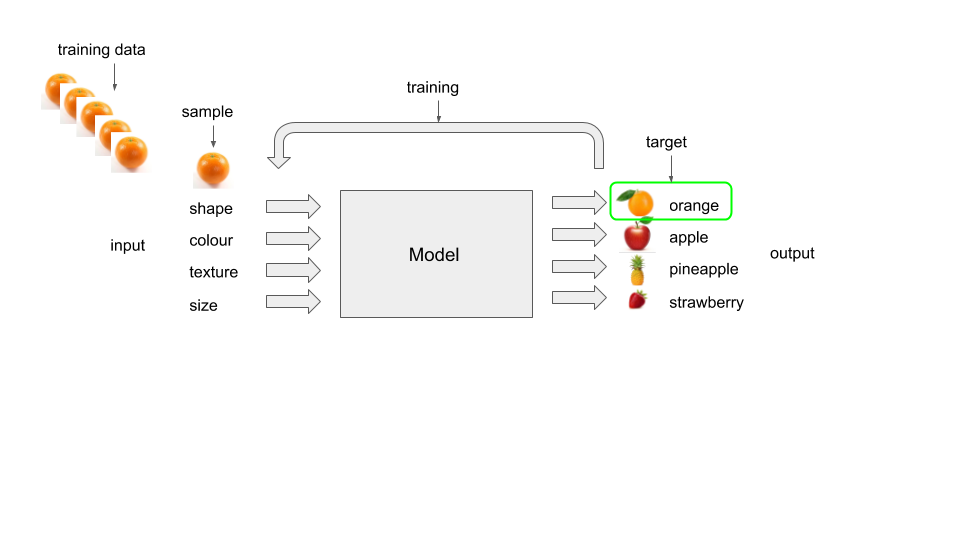
\includegraphics[width=1.0\textwidth, height=0.4\textwidth]{supervised_learning}
	\captionsetup{justification=centering}
	\caption{A machine learning model trained using supervised learning. The task of this model is to map input features to output categories, predict a type of fruit given an image.}
\end{figure}

\noindent Features can be continuous valued or discrete, where discrete values are referred to as categorical variables. Outputs can also be continuous or discrete, where discrete outputs are known as classes. Example input-output pairs comprise a training dataset which is represented as \begin{math} D = \{(x_i, \; y_i)\}_{i=1}^N \end{math}, where \begin{math} x_i \end{math} is the input feature and \begin{math} y_i \end{math} is its expected output label. The model has to learn a general mapping from input features to output labels. \par

\noindent In the fruit example, the model will attempt to build decision boundaries between fruit classes in the feature space.\ We can visualise this process in a $2$-dimensional ($ 2D $) setting using two fruit features, say shape and colour. Figure 2.2 shows an example of synthetically generated samples in this $ 2D $ feature space and a potential decision boundary.

\begin{figure}[H]
   	\centering
    	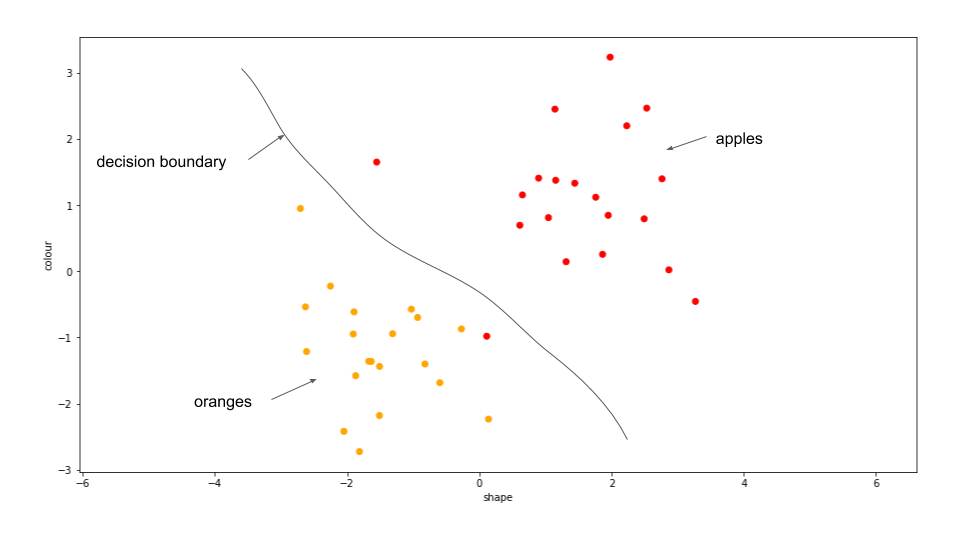
\includegraphics[width=0.6\textwidth, height=0.4\textwidth]{oranges_and_apples_decision_boundary}
	\captionsetup{justification=centering}
	\caption{A decision boundary between two classes, apples and oranges. The model constructs this curve by learning the feature characteristics corresponding to each class.}
\end{figure}

\noindent Data is assumed to be generated by the same underlying process, and would be either: independent and identically distributed (IID), or dependent. In the context of IID data, samples are independent and therefore order invariant; while in the context of dependent data, samples are dependent and order matters.\ The class of data can determine the best choice of model for prediction. \par

\noindent Available labelled data is typically subdivided into three sets: training, validation and test. The training set provides in-sample data -- input-output pairs which are exposed to the model during training and used to update its parameters. The validation set approximates out-of-sample data used to adjust model architecture, as well as hyperparameters (meta model parameters which configure its operation). The test set is used to assess the model's prediction performance after training and hyperparameter tuning are complete. These results establish an objective measure of the model's utility.  \par

\noindent An objective function is used to measure the prediction performance of a model during training, and can compute an error or reward signal.\ When the objective computes an error it is called a loss function, and measures the difference between the model's predicted output and the target output (the labels in the training set). As the model parameters are updated during training, the loss value changes and produces a multidimensional loss surface. The training algorithm tries to minimise this loss using a method of optimisation, such as Bayesian, evolutionary or first order. When the objective computes a reward it is called a reward function, and is often used when a sequence of steps is required to complete a task \unskip ~\citep{murphy2012machine}. The training algorithm tries to maximise the reward, which is typically applied in reinforcement learning settings. The reader is referred to \unskip~\citep {sutton2018reinforcement} for a complete introduction. \par

\noindent A popular method of optimisation is gradient descent, which tries to descend to the lowest region of the loss surface: the global minimum. Model parameter updates are computed based on partial derivatives of the loss, with respect to the individual parameters.\ The size of the update is dependent on the magnitude of the gradient of the loss i.e. the steeper the gradient, the larger the update. A training algorithm uses gradient descent to guide the loss toward the global minimum, but in practice a local minimum is usually the best that can be achieved. In doing so the algorithm attempts to optimise the model, such that it can estimate the underlying distribution of the data, enabling it to perform inference. \par

\noindent During training, mini-batch optimisation is often used along with gradient descent to update model parameters. In mini-batch optimisation the training set is divided into batches, where model parameters are updated after a mini-batch has been processed.\ This is in contrast to stochastic gradient descent where parameters are updated per sample, and batch gradient descent where parameters are updated after a run through the entire training set. Mini-batch optimisation is both robust to convergence (not as susceptible to local optima), and compute efficient. \par

\noindent The supervised learning training algorithm is expressed as follows: \par 

\bigskip

\begin{algorithm}[H]
	\SetAlgoLined
	\textbf{Input} 
	Training set \begin{math} D = \{(x_i, \; y_i)\}_{i=1}^N \end{math} of input features and output labels\;
	Intialise parameters $w \in \mathbb{R}^d$, for model \begin{math} M(w) \end{math} // e.g. random normal initialisation \\
	\For{Epoch \begin{math} k =  1 \dots \; K  \end{math}}{
  		\begin{math} B \gets sample(D, s) \end{math} // sample mini-batch of size \begin{math} s \end{math} \\
	 	\For{(x, y) \begin{math} \in B \end{math}}{
     			\begin{math} y' \gets predict(x, \; y') \end{math} // predict label for sample \\
			\begin{math} e \gets y' - y \end{math} // compute loss
     			}
		$ w \gets w - \lambda \cdot \nabla_{w} J_{e}(w) $ // gradient descent update of model with respect to loss $ e $, \\  // where $ \lambda$  is the learning rate, and $ J_{e}(w) $ is the partial derivative of parameter $ w $ 
	}
	\caption{Supervised Learning}
\end{algorithm}


%********************************** %Second Section  **************************************

\section{Deep learning models}

Deep learning models have become popular for classification and regression tasks, and machine learning tasks in general.\ The reason for this is that deep models solve a major problem with shallow models, which is to select the best features with which to represent raw input samples \unskip ~\citep{Goodfellow-et-al-2016}.\ The problem of feature selection has resulted in a methodology used during shallow model development, called feature engineering.\ It includes techniques such as bucketing, crossing, hashing and embedding.\ These techniques are designed to build feature representations that will result in high classification and regression accuracy.\ Deep models attempt to discover optimal representations automatically during training, hence their superior performance on a number of machine learning tasks. \par

\noindent Multilayer perceptrons (MLPs) are deep learning models implemented as feed-forward neural networks, consisting of $N$ layers applied to an input vector $ x $.\ These models compute unnormalised scores, known as logits, for each of the possible outputs.\ They construct a composition of nonlinear functions which describe an analytical definition of the generative process of the data used to train them. The utility of composition is what gives them the capability needed to model complex datasets. MLPs achieve nonlinear expressiveness with the use of nonlinear activation functions, such as the ReLU, Sigmoid and Tanh functions.  \par

\noindent MLPs generate an output by executing a number of steps in what is called the forward pass, where each step is represented as a layer. A basic MLP may consist of three layers: an input, hidden and output layer. It uses a hidden layer comprised of neurons (nodes) to generate an activation (output) per node.\ Each node computes a linear combination of inputs from the previous layer, and then transforms the result using a nonlinear activation function.\ The set of node outputs is a hidden vector representation, which is passed to the following layer as input. The output layer generates a logit, using a linear combination of inputs from the hidden layer, see Figure 2.2. The more hidden layers the model has, the deeper it is.

\begin{figure}[H]
   	\centering
    	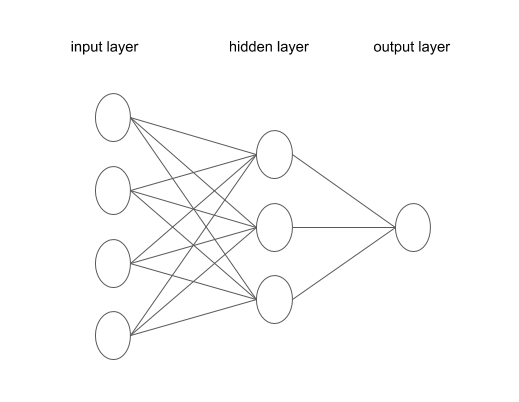
\includegraphics[width=0.5\textwidth, height=0.3\textwidth]{multilayer_perceptron}
	\captionsetup{justification=centering}
	\caption{A basic MLP consisting of an input, hidden and output layer. The model can comprise an arbitrary number of hidden layers, containing an arbitrary number of nodes.}
\end{figure}

\noindent The forward pass can be expressed as follows:
\begin{subequations}
	\begin{gather}
		f_0 = x \\
		f_i=\sigma_i(W_{hi}f_{i - 1} + b_{hi}) \quad i \in [1, \; N] \\
		f_o = W_{o}f_N + b_o
	\end{gather}
\end{subequations}

\noindent Where $ f_0 $ is the input layer, the features of input vector $ x \in \mathbb{R}^{m_0} $. $ f_i $ is a hidden layer output vector of size $ m_i $, $ f_{i - 1} $ is the input vector from the previous layer of size $ m_{i-1} $. $ W_{hi} \in \mathbb{R}^{m_i \times m_{i - 1}} $ is a matrix of hidden layer parameters, $ b_{hi} \in \mathbb{R}^{m_i} $ is a vector of hidden bias parameters. $ \sigma_i \in \mathbb{R}^{m_i} $ a vector nonlinear activation functions. $ f_o $ is the output layer, a vector of logits $ y \in \mathbb{R}^o $, $ f_N $ is the final input vector of size $ m_{N} $. $ W_{o} \in \mathbb{R}^{m_N \times m_o} $ is a matrix of output layer parameters, $ b_{o} \in \mathbb{R}^{m_o} $ is a vector of output bias parameters.

\noindent Loss functions are used to train deep models under a supervised learning paradigm.\ The loss function is minimised with gradient descent, which in the case of MLPs makes use of a process called backpropagation.\ This process involves the computation of first order partial derivatives, and the adjustment of the parameters in a direction and magnitude relating to their respective derivative. In a network with $ N $ layers, the gradient for the respective parameter in layer $ i $ is given by:
\begin{subequations}
	\begin{gather}
		\frac{\partial E} {\partial W_i} = \frac{\partial E} {\partial z_N}\frac{\partial z_N} {\partial z_{N - 1}}  \dots \frac{\partial z_{i + 2}} {\partial z_{i + 1}}\frac{\partial z_{i + 1}} {\partial W_{i}} \\
		\frac{\partial E} {\partial b_i} = \frac{\partial E} {\partial z_N}\frac{\partial z_N} {\partial z_{N - 1}}  \dots \frac{\partial z_{i + 2}} {\partial z_{i + 1}}\frac{\partial z_{i + 1}} {\partial b_{i}}
	\end{gather}
\end{subequations}

\noindent where $ E $ is the loss function, $ W_i $ is parameter matrix for layer $ i $, $ z $ is the layer output, and $ b_i $ is the bias vector at layer $ i $. The matrix $ \frac{\partial z_{i + 1}} {\partial W_i} $ is called a Jacobian matrix.\ The Jacobian matrix contains the partial derivatives of the layer-specific parameters, with respect to the loss contributed by each parameter to the overall output error. It summarizes all the ways in which changing the matrix $ W_i $ by a small amount will influence the output $ z_{i + 1} $. The matrix is expressed as follows: \par
\begin{equation}
	\renewcommand\arraystretch{2}
	J = \begin{bmatrix}
        		\frac{\partial z^1}{\partial W^1} & \frac{\partial z^2}{\partial W^1} & \cdots & \frac{\partial z^m}{\partial W^1} \\
           	\frac{\partial z^1}{\partial W^2} &\frac{\partial z^2}{\partial W^2} & \cdots & \frac{\partial z^m}{\partial W^2} \\
           	\vdots & \vdots & \ddots & \vdots \\
           	\frac{\partial z^1}{\partial W^n} & \frac{\partial z^2}{\partial W^n} & \cdots & \frac{\partial z^m}{\partial W^n} \\
        \end{bmatrix}
\end{equation}

\medskip
\noindent Different schemes are used to initialise layer parameters $ W_i $ and $ b_i $. These schemes are sensitive to the choice of activation function, $ \sigma_i $, used.\ Sigmoid and Tanh functions can saturate if parameters are intialised with values that are too large, or can die if intialised with values which are too small, which in turn can lead to exploding and vanishing parameter gradients. In order to overcome this problem Xavier intialisation \unskip ~\citep{glorot2010understanding} is used, which tries to scale the parameters by the number of layer inputs and outputs.\ This limits the variance of layer outputs and helps stabilise gradient updates.\ When the ReLU activation is used He intialisation \unskip ~\citep{he2015delving}, a modification of Xavier initialisation, is commonly applied. \par

\noindent Together the forward pass algorithm and backpropagation implicitly allow the automatic discovery of the most meaningful representations used to generate model output.\ We refer the reader to \unskip ~\citep{Goodfellow-et-al-2016} for a review on loss functions, as well as a more detailed discussion on the forward pass and backpropagation. 


%********************************** %Convolutional Networks  **************************************

\subsection{Convolutional networks}

MLPs suffer from an explosion of parameters \unskip ~\citep{krizhevsky2012imagenet}. In an MLP layer, all features of an input vector are fully connected to all other features when computing the layer output. The outputs of a layer are then all fully connected to each other in the following layer. This interconnectedness causes the number of model parameters to grow exponentially in the number of input features. For example, a feed-forward network with two hidden layers consisting of $ 512 $ and $ 256 $ neurons respectively, an output size of $10$, and an input vector of shape $ \left [ \begin{matrix} 200 \times 1 \end{matrix} \right] $, ends up with a total of $ 236,810 $ parameters. This can cause a problem with high-dimensional input vectors such as images, where inputs may consist of a $ 3D $ input volume. MLPs may also need to be composed of a number of layers in order to produce satisfactory prediction performance when presented with high-dimensional inputs.\ In such a scenario, parameters can number in the millions, resulting in a model that is computationally inefficient to train. \par

\noindent MLPs are also not able to take direct advantage of structure in data.\ When images are represented as a matrix, common shapes (features) may appear in a regular composition. For example, different cars may appear regularly as a compositions of rectangles and circles. The inner product operator applied between the input (which is typically flattened into a vector) and layer parameters of an MLP, destroys the spatial information of the data, making the task of learning distributions of features harder. As a result, in order to possess sufficient learning capacity that adequately models variance in structural representations, MLPs need to be larger and despite this may still produce poor prediction performance. \par

\noindent Convolutional networks (CNs) have been developed to overcome both the above mentioned problems experienced by MLPs. CNs make use of the convolutional operator instead of the inner product operator by using a filter, a matrix with trainable parameters. This process generates a latent feature map which is used in subsequent layers in the network, see Figure 2.4. Latent feature maps may capture structural patterns in data, building simple intermediate representations. CNs compose these representations into more sophisticated representations in subsequent layers. \par 

\begin{figure}[H]
	\centering
	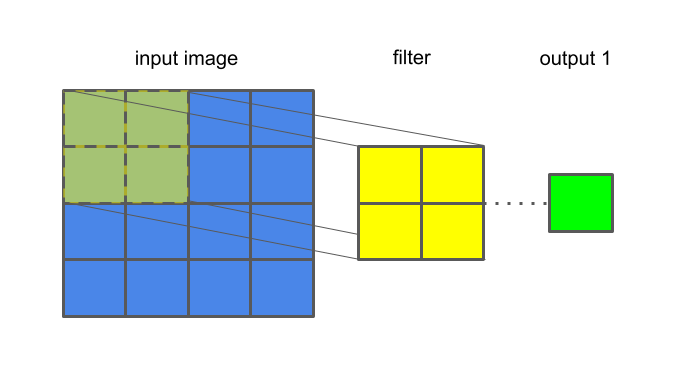
\includegraphics[width=0.33\textwidth, height=0.25\textwidth]{convolution1}\hfill
	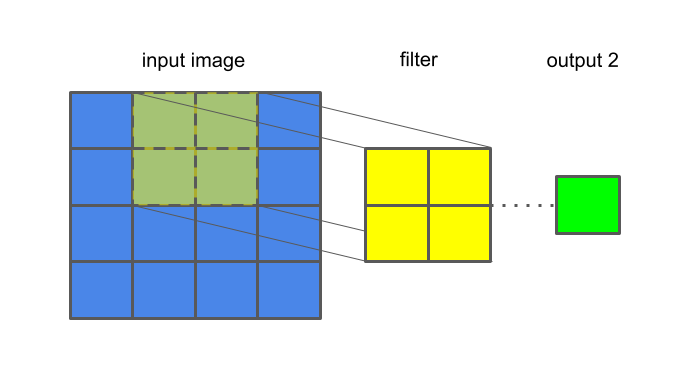
\includegraphics[width=0.33\textwidth, height=0.25\textwidth]{convolution2}\hfill
	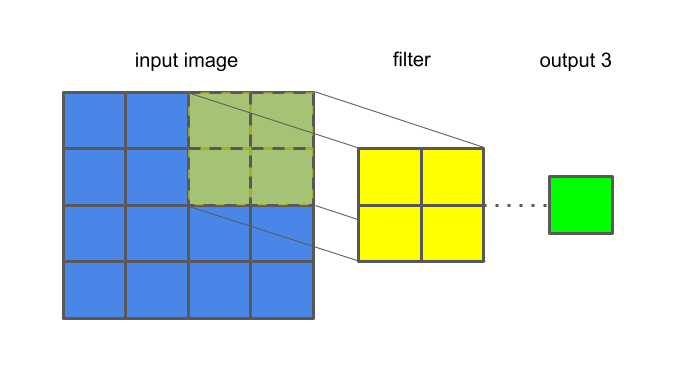
\includegraphics[width=0.33\textwidth, height=0.25\textwidth]{convolution3}
	\captionsetup{justification=centering}
	\caption{A convolutional operation taken between an input image and a filter. The filter slides across the image, and at each step computes a summary of that location as a single value.}
\end{figure}

\noindent The convolutional operator allows CNs to capture translation invariance in inputs, due to filter parameter sharing \unskip ~\citep{simonyan2014very}.\ Translation invariance is achieved when a CN layer generates an intermediate representation that is consistent under transformation. For example, if a different image of  car is used as input, and the car is located in a different position, that would lead to a consistent feature map representation being generated, see Figure 2.5. This property allows CNs to model the distribution of features using fewer parameters and smaller datasets. \par 

\begin{figure}[H]
   	\centering
    	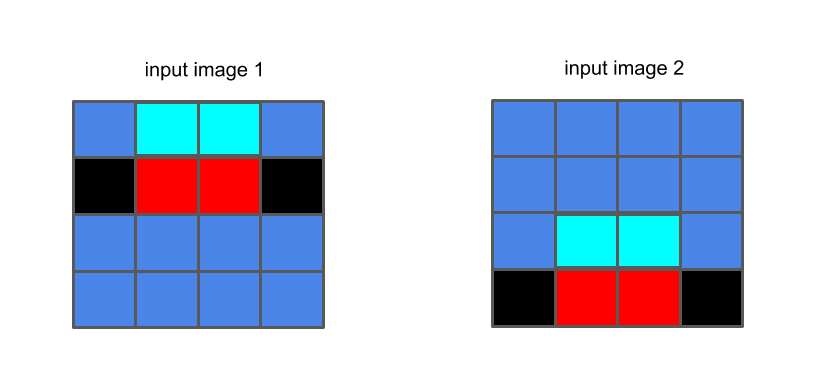
\includegraphics[width=0.6\textwidth, height=0.3\textwidth]{translation_invariance}
	\captionsetup{justification=centering}
	\caption{Two images of the same object, in different locations. Filter parameter sharing enables input translation invariance. The CN should predict "car" on both occasions.}
\end{figure}

\noindent The trade off one makes when using CNs is reduced flexibility in modelling complex decision boundaries.\ To mitigate this trade off, CNs are often implemented with a final set of fully connected layers, which enable the expressiveness required for accurate prediction, see Figure 2.6. \par

\begin{figure}[H]
   	\centering
    	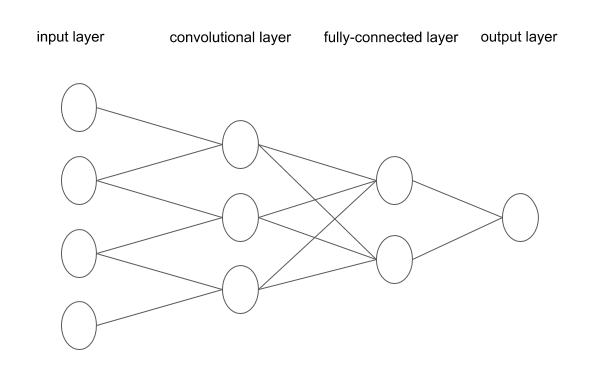
\includegraphics[width=0.5\textwidth, height=0.3\textwidth]{convolutional_network}
	\captionsetup{justification=centering}
	\caption{A basic CN consisting of an input, convolutional layer, fully connected layer and output layer.}
\end{figure}

\noindent In the following we discuss the CN forward pass. \par

\noindent \textbf{Convolutional layers.} Convolutional layers rely on filters that are small spatially (along width and height), and extend through the full depth of an input volume. During the forward pass, each filter is convolved across the width and height of the input volume, where the element-wise dot product is computed between the entries of the filter and the input at a particular position. A $ 2D $ feature map is generated, that gives the responses of that filter at every spatial position of the input. Every convolutional layer has a set of filters, and each of them produces separate $ 2D $ feature maps, which are then stacked along the depth dimension to produce an output volume \unskip ~\citep{DLIndaba2017}. \par

\noindent  The size of the output volume is controlled by the hyperparameters of the convolutional layer, namely the filter size (kernel), number of filters (channels), stride, padding, and dilation. The kernel size defines the width and height of the kernel, which is often square, and the filter is the set of kernels that is the same size as the depth of the input volume, see Figure 2.7. The number of channels controls the output volume depth. The stride defines the number of entries by which the filter will move when convolving it along the input volume, see Figure 2.8 and Figure 2.9. Padding refers to the number of $ 0 $ entries added to the input volume along the width and height dimensions. It can be used to ensure that the output volume has the same width and height as the input volume. Dilation introduces spaces between the filter parameters, and is used to increase its receptive field, see Figure 2.10. \par

\begin{figure}[H]
   	\centering
    	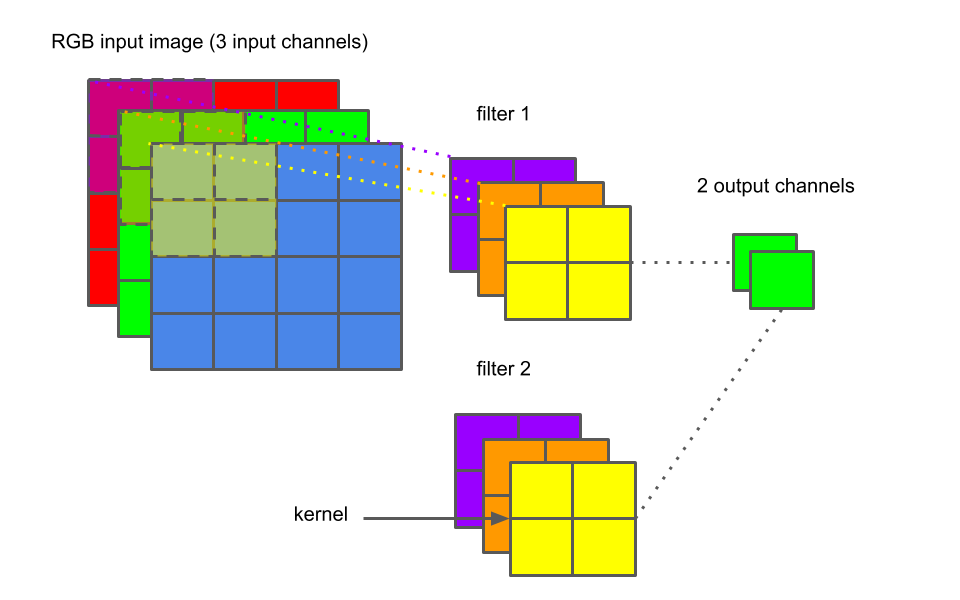
\includegraphics[width=0.6\textwidth, height=0.3\textwidth]{channels}
	\captionsetup{justification=centering}
	\caption{A $ 3D $ input image with 3 input channels. A kernel size of $ 2 $ is used, where the filter depth is the same as the number of input channels $ 3 $. Using $ 2 $ filters produces $ 2 $ output channels.}
\end{figure}

\begin{figure}[H]
	\parbox{.5\linewidth}{
   		\centering
    		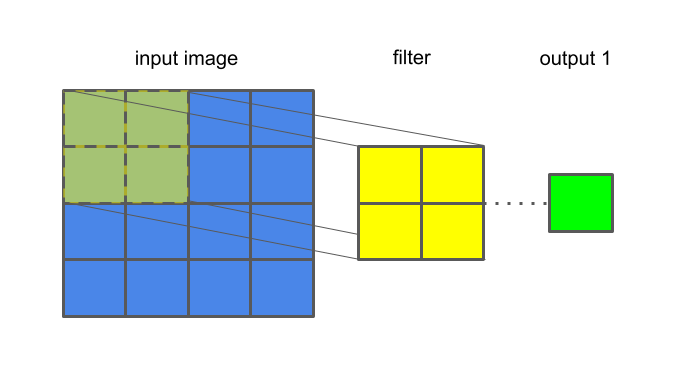
\includegraphics[width=0.45\textwidth, height=0.2\textwidth]{convolution1}
		}
	\hfill
	\parbox{.5\linewidth}{
   		\centering
    		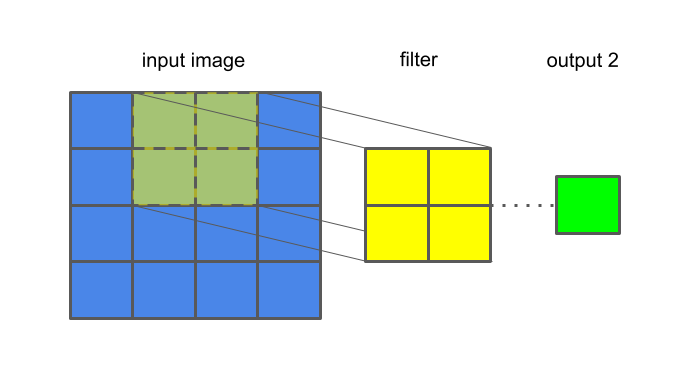
\includegraphics[width=0.45\textwidth, height=0.2\textwidth]{convolution2}
		}
	\captionsetup{justification=centering}
	\caption{Convolution operation with a stride of 1.}
	
	\parbox{.5\linewidth}{
   		\centering
    		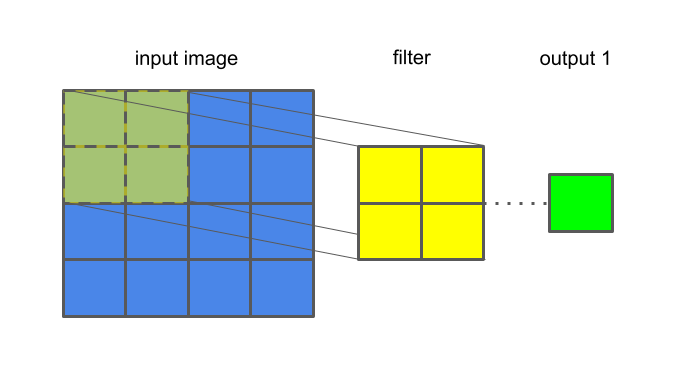
\includegraphics[width=0.45\textwidth, height=0.2\textwidth]{convolution1}
		}
	\hfill
	\parbox{.5\linewidth}{
   		\centering
    		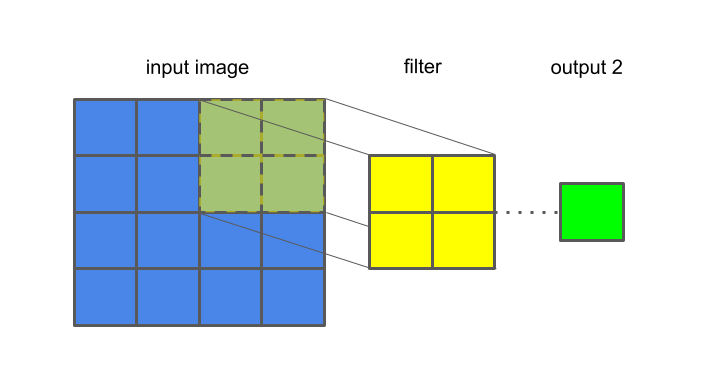
\includegraphics[width=0.45\textwidth, height=0.2\textwidth]{stride_of_2}
		}
	\captionsetup{justification=centering}
	\caption{Convolution operation with a stride of 2.}
\end{figure}

\begin{figure}[H]
   	\centering
    	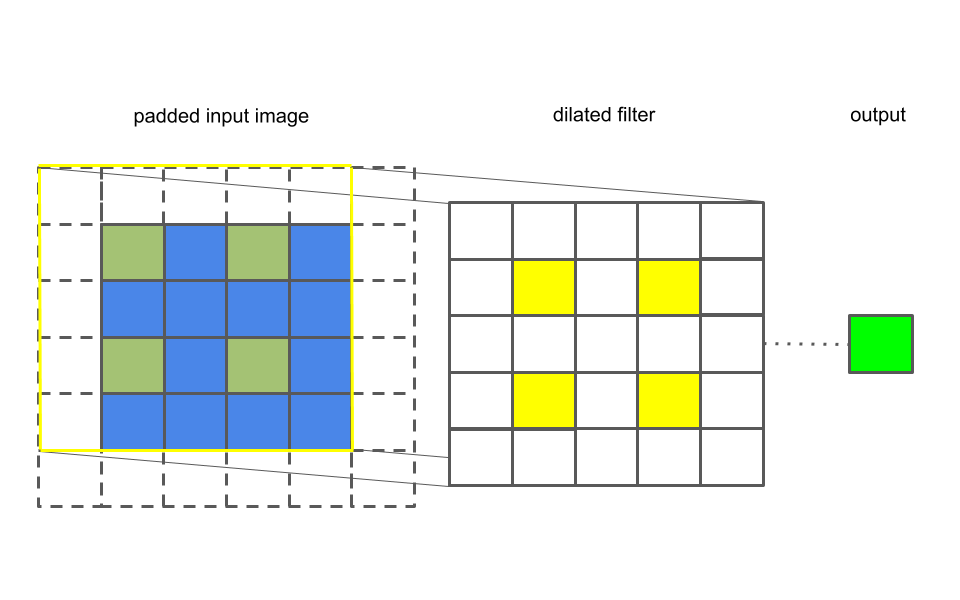
\includegraphics[width=0.6\textwidth, height=0.3\textwidth]{padding_and_dilation}
	\captionsetup{justification=centering}
	\caption{An input image with a padding of $ 1 $, convolved with a filter with a dilation of $ 2 $.}
\end{figure}

\noindent Convolution of an input volume $ X $ with a single filter $ W $ is given by: 
\begin{equation}
	O_{ij}^{d} = \sum_{a=0}^{f_w - 1}\sum_{b=0}^{f_h - 1}\sum_{c=0}^{d_i - 1}W_{a,b,c,d_o}X_{i+a,j+b,c}^{pad}  + b_{d_o} 
\end{equation}

\noindent where $ O_{ij}^d $ is the value of the output volume at position $ i, \; j $ of feature map $ d $. $ W_{a,b,c,d} \in \mathbb{R}^{f_wf_hd_id_o} $ is set of filters with kernel size $ f_w \times f_h $, number of input channels $ d_i $, and number of output channels $ d_o $. $ X^{pad} $ is the padded input volume and $ a, \; b, \; c $ are indices into the volume dimensions. $ b \in \mathbb{R}^{d} $ is a bias vector. \par

\noindent \textbf{Pooling layers.} A pooling layer is used to reduce the spatial size of the representation, in order to reduce the number of parameters in the network.\ Pooling layers provide latent features deeper in the network with a larger receptive field. In particular, pooling gives deeper latent features much larger receptive fields so that they can effectively combine smaller features together. Pooling layers apply some $ 2D $ aggregation operation (usually a max, but others like average may also be used) to local regions of the input volume. A pooling layer has no trainable parameters itself. \par

\noindent \textbf{Fully connected layers.} In order to compute the output of a CN, one or more fully connected layers are required to flatten the output volume of the last convolutional layer. These layers perform the same functions as an MLP to compute an output vector. \par

\noindent \textbf{Convolutional backpropagation.} Computing parameter updates for convolutional filters follows the same first order differential procedure used in backpropagation for MLPs. Assuming a loss function $ E $, and having computed the derivative of this loss up to the output of the convolutional layer, $ \frac{\partial E} {\partial O} $, in order to update the parameters the convolutional layer, we require the derivative of $ E $ with respect to the weights and biases of the convolutional layer. We also require the derivative with respect to the input to the current layer $\frac{\partial E} {\partial X}$, and use this when computing the error to pass back to the previous layer. \par

\noindent The required derivatives are:
\begin{subequations}
	\begin{gather}
		\frac{\partial E} {\partial b} = \frac{\partial E} {\partial O}\frac{\partial O} {\partial b} \\
		\frac{\partial E} {\partial W_{a,b,c,d}} = \sum_{i=0}^{O_w - 1}\sum_{j=0}^{O_h - 1}\frac{\partial E} {\partial O_{ij}^{d}}\frac{\partial O_{ij}^d} {\partial W_{a,b,c,d}} \\
		\frac{\partial E} {\partial X_{m,n,c}^{pad}} = \sum_{i=0}^{O_w - 1}\sum_{j=0}^{O_h - 1}\sum_{d=0}^{D - 1}W_{m-i,n-j,c,d}\frac{\partial E} {\partial O_{ij}^{d}}
	\end{gather}
\end{subequations}

%********************************** %Recurrent Networks **************************************

\subsection{Recurrent networks}

An IID dataset is order invariant, because the probability of seeing one data point in no way influences the event of seeing another. Practically, this means shuffling the data when training a model has no influence on prediction performance.\ Some data is however dependent, and when training a model the order of the data points matters. Such data is presented as a sequence which is broken into steps, where each step is influenced by the steps before it. \par

\noindent An example of dependent data is the daily temperature of Cape Town over a year. This sequence can be broken into steps, where each step is the daily high in degrees Celsius. The temperature on day $ t $ is influenced by the temperature on the preceding days, $ t - 1, \; t - 2, \; \dots \; t - n $. If we try to predict the temperature one day into the future, it is reasonable to believe that if the daily high on day $ t - 2 $ was mild, and the daily high on day $ t - 1 $ was warm, the daily high on day $ t $ may be hot. \par
 
\noindent Text expressed in natural language is another example of sequential data. This data is arranged in sentences which are comprised of sequences of words. Each word represents a step in the sequence, and if we try to predict the word at step $ t $, it may be useful to have context of the words at $t -1$ and $t - 2$. For example in the sentence, "I think, therefore I ...", we would want to predict "am" as the next word. \par

\noindent In the task of one step ahead prediction, we build models that attempt to estimate a probability distribution over a sequence. This distribution estimates the likelihood of seeing a data point given a preceding sequence. Formally we estimate a conditional distribution given a sequence. \par 

\noindent The conditional distribution is defined as follows:
\begin{equation}
	\begin{split}
		\Pr( x_t | x_{t - 1},  x_{t - 2}, \dots,  x_{t - n} ) & = \Pr(x_t | x_{t - 1}) \Pr(x_{t - 1}| x_{t - 2}) \; \dots \; \Pr(x_{t - n - 1}| x_{t - n}) \Pr(x_{t-n}) \\
		& = \prod_{t=1}^N \Pr(x_t | x_{t - 1})
	\end{split}
\end{equation}

\noindent Recurrent networks (RNs) estimate the conditional distribution of dependent data points from sequential input by modelling a summary of previous data points. This summary is defined as an internal state of the model, which contains outputs from previous sequence steps combined with a recurrent parameter matrix using an matrix-vector product operator.\ RNs thus extend feed-forward networks like MLPs and CNs by directly incorporating sequential dependencies between data in the model, see Figure 2.11. \par

\begin{figure}[H]
   	\centering
    	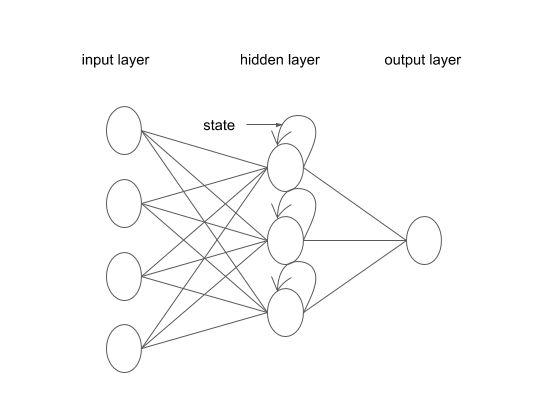
\includegraphics[width=0.5\textwidth, height=0.3\textwidth]{recurrent_network}
	\captionsetup{justification=centering}
	\caption{A basic RN consisting of an input, hidden and output layer. An internal state is added to hidden layer nodes which tracks previous output. This state is summed with the node output.}
\end{figure}

\noindent Additional context applied to RN prediction is made at the expense of a higher number of model parameters. The increase in parameters is linear in the number of sequence steps considered in the context summary. Practically this means a truncated sequence is used to provide context during training, to keep computation tractable. \par

\noindent In the following we discuss the RN forward pass. \par

\noindent \textbf{Recurrent layers.} RNs build context by generating a representation of a window of data samples. This representation is defined as a state vector, which is added to a hidden vector and bias of a layer within the network. The layer output is then passed through a nonlinear activation before being passed to the next layer. RN layers are comprised of cells, which contain an internal state, hidden output and a bias \unskip ~\citep{DLIndaba2018}. An RN cell can thus be defined as follows: 
\begin{equation}
	h_t = \sigma(W_{hh}h_{t-1} + W_{xh}x_t + b)
\end{equation}

\noindent where $h_t$ is the cell output, and added to the state vector as context for the following sequence step. $\sigma$ is a nonlinear activation function, $W_{hh}$ contains the recurrent parameters, $W_{xh}$ contains the non-recurrent parameters, $x_t$ is the input and $b$ is the bias. $h_t$ is then used as input to a fully connected layer for prediction at every step, which is given by:
\begin{equation}
	y_t = \sigma(W_{hy}h_{t} + b)
\end{equation}

\noindent \textbf{Backpropagation through time.} RNs are trained using a method called backpropagation through time (BPTT),  a gradient-based process that updates recurrent parameters by unrolling cell outputs over a window of sequence steps.\ Parameter gradients are computed at each step with respect to the error generated at that prediction step. The error signal generated is backpropagated through the RN layer to adjust the cell state, hidden and bias parameters, by computing their first order partial derivatives. In practice, a fixed sequence length is decided upfront for updating cell parameters, a process called truncated BPTT, which has compute resource advantages. Standard backpropagation is used for non-recurrent parameter updates. \par

\noindent The gradient of the loss function $ E_t $ at time $ t $ with respect to $ W_{hh} $ is a function of the current hidden state and model predictions $\hat{y_t}$ at time $ t $:  
\begin{equation}
	\frac{\partial E_t} {\partial W_{hh}} = \sum_{k=0}^{t}\frac{\partial E_t} {\partial \hat{y_t}}\frac{\partial \hat{y_t}} {\partial h_t}\frac{\partial h_t} {\partial h_k}\frac{\partial h_k} {\partial W_{hh}}
\end{equation}

\noindent One problem experienced by RNs is the multiplicative effect of state vector derivates throughout sequence-time. This problem can be seen in the following expression:
\begin{equation}
	\frac{\partial h_t} {\partial h_k} = \prod_{j=k+1}^t\frac{\partial h_j} {\partial h_{j-1}}
\end{equation}

\noindent This multiplicative operation causes small gradients to become progressively smaller as the sequence window becomes larger, or large gradients to become much larger. This is called the vanishing or exploding gradient problem and has lead to the development of RN variant models such as long short-term memory \unskip ~\citep{hochreiter1997long} and gated recurrent units \unskip ~\citep{cho2014learning}.


%********************************** %Third Section  **************************************

\section{Regularisation}

Model over-parameterisation can lead to overfitting on in-sample data.\ This is because the degrees of freedom available to estimate a function allow very complex nonlinear functions to be discovered, where these nonlinear functions are not representative of the generative process of the data. In fact, the model may end up fitting to the noise in the dataset. Overfitting results in poor generalisation to new data. This problem forms part of the broader bias/variance trade off, specifically high model variance due to over parameterisation. Deep learning models are particularly sensitive to overfitting given the high number of parameters present within the model. Regularisation techniques are used to improve the generalisation capability of deep models. \par

\noindent \textbf{L1 and L2 regularisation.} Lasso (L1) \unskip ~\citep{tibshirani1996regression} and Ridge (L2) \unskip ~\citep{hoerl1970ridge} regression are two common approaches to prevent overfitting, by adding a term to the loss that penalises the model if it becomes too complex. They are defined as follows:
\begin{subequations}
	\begin{gather}
		loss_{L1} = loss + \lambda\sum_i\abs{w_i}  \\
		loss_{L2} = loss + \lambda\sum_iw_i^2
	\end{gather}
\end{subequations}

\noindent L1 regularisation has the effect of forcing some parameters to shrink to 0, effectively removing them from the model. L2 regularisation has the effect of preventing any of the parameters from becoming too large and overpowering the others. \par

\noindent \textbf{Early stopping.} As deep models are trained using a supervised learning paradigm, the model training accuracy gradually increases. As training continues, the model validation accuracy gradually increases, and then begins decreasing. At this point the model has begun overfitting the training data.\ If the model continues training, the validation accuracy may continue decreasing, and should the model then be tested, the resulting test accuracy may be lower than the training accuracy. Early stopping is a technique used to try to prevent overfitting. Once the training and validation accuracies begin to diverge, training continues for a few more epochs, and if the divergence persists, training is terminated. \par

\noindent \textbf{Dropout.} During training, nodes in a deep model can generate redundant latent features that overfit to the training data.\ Dropout is a technique that is used during training to zero out a randomly selected proportion of neurons in the layer of a deep model. This has the effect of removing partial dependence between nodes deeper within the network, preventing complex co-adaptation of hidden layers, and resulting in more independent latent features \unskip ~\citep{hinton2012improving}. These features produce a more robust representation of the generative process of the data, allowing greater model generalisation to out-of-sample data. \par

\noindent \textbf{Batch normalisation.} Deep models are composed of parameterised layers. When the parameters of these layers are adjusted during training using mini-batch optimisation, each data point within the batch contributes to the model output individually, however the error is aggregated across the entire batch. This results in a shift in the distribution of node output for each layer, a problem known as internal covariate shift. Covariate shift makes it difficult for the model to estimate the underlying generative distribution of the data, and batch normalisation has been proposed as a technique to compensate for this problem. \par

\noindent Batch normalisation solves two other problems experienced during deep model training, namely nonlinearity saturation and weight initialisation sensitivity. It does this by computing layer-specific moving average estimators of the batch mean and standard deviation.\ Each layer's node output is then modified by these statistics before being passed onto the following layer. Batch statistics at training time are then aggregated into global population statistics during test time.\ Batch normalisation's application shortens the required model training time, and can result in better prediction performance. 


%********************************** %Fourth Section  **************************************

\section{Language Models}

\noindent Language models are a set of vector representations for the words in a language. They capture statistical correlations between the words, and in so doing build an understanding of semantic meaning. They encode this meaning in a word vector space, where for example the vectors for the words "film" and "character" may be collocated, given they share semantic meaning. Language models are often trained using RNs on large sequential text datasets, the following presents a discussion on their development. \par

\noindent Word2Vec, introduced by Mikolov et al. \unskip~\citep{mikolov2013distributed}, is an algorithm for training distributed representations of words.\ The skip-gram model \unskip ~\citep{mikolov2013efficient} is one of the models used by Word2Vec to generate word vectors from very large text corpora (more than a billion words). The model essentially takes a centre word, and then tries to predict the probability of seeing a context word to the right or left of the centre word. This context window can also be longer than one word. The skip-gram model uses the hierarchical softmax loss function \unskip~\citep{morin2005hierarchical} for classification (a computationally efficient approximation of the full softmax) and employs the subsampling of frequent stop words such as “in”, “the”, and “a”. The continuous bag of words (CBOW) model is an alternative approach to the skip-gram model.\ Here the model tries to predict a target word, given a sequence of context words. CBOW has the advantage of being faster to train and producing better representations for more frequent words. \par

\noindent GloVe, by Pennington et al.\unskip~\citep{pennington2014glove}, is another unsupervised learning algorithm for generating word vectors. This model generates word vectors using the co-occurrence statistics of words in a text corpus. The corpus is viewed as a global statistics space, and the model begins with a pass over the entire corpus to generate a co-occurrence matrix of words against all other words in the corpus. GloVe thus captures both global and local statistics of a corpus, compared to Word2Vec which only captures local corpus statistics.\ GloVe then attempts to model the co-occurrence statistics between words using a neural network that takes two words as input and scores the co-occurrence statistic as output. The training procedure minimises a logarithmic squared error loss that incorporates both global and local corpus statistics. The distributional representation of word embeddings that GloVe employs, allows it to outperform Word2Vec on word analogy, word similarity, and named entity recognition tasks. It is therefore the chosen word embedding method used in this thesis. \par

\noindent A number of alternative approaches to building language models have become popular, including FastText \unskip~\citep{bojanowski2016enriching}, BERT \unskip~\citep{vaswani2017attention} and ELMo \unskip~\citep{peters2018deep}. FastText takes advantage of modelling every word as a combination of character n-grams, providing representations for rare and unseen words. BERT and ELMo take advantage of contextual representations of words, generating on-the-fly representations for words given a sequence of words instead of returning a precomputed word representation by index lookup.\ These representations are superior at capturing semantic information than static representations.\ The need for sequences of words to generate entity representations makes BERT and ELMo unsuitable for use in latent feature modelling.


%********************************** %Fifth Section  **************************************

\section{Summary}

Supervised learning is a paradigm used to train ML models where target output is provided with corresponding input.\ This paradigm allows models to build an input-output map that approximates the underlying data distribution.\ The effectiveness of this mapping is heavily dependent on the input representation of samples, known as features. \par

\noindent We can take advantage of automatic representation construction using deep learning models. Deep models differ from their shallow counterparts by computing latent feature representations directly from the data. This has been shown to be more effective than manually constructing feature representations using techniques such as bucketing, crossing, hashing and embedding. CNs solve the over parameterisation problem in MLPs, and simultaneously take advantage of spatial structure present in data samples. RNs provide context of previous samples using state vectors when modelling sequential data. Both these approaches have been applied successfully in classification and regression tasks. \par

\noindent Deep models can overfit data and as a result generalise poorly to test datasets.\ A number of approaches have been used to address this problem, including lasso and ridge regression, early stopping and dropout. Batch normalisation has proved particularly effective at regularisation as it compensates for the covariate shift experienced by deep models during training. In addition, batch normalisation also speeds up training time, and makes deep models less sensitive to weight initialisation. \par

\noindent Language models build an understanding of the meaning of words in a language.\ They are constructed using the distributed representation of words or distributional representation of words hypotheses, and trained using RNs on large sequential text datasets. Language models generate word vectors, embedded in a word vector space, which can be used in downstream ML tasks. 
